% !TeX root = ../main.tex
\label{sec:definitions}

% reduce display equation skip
 \setlength{\abovedisplayskip}{4pt}
 \setlength{\belowdisplayskip}{4pt}
 \setlength{\textfloatsep}{4pt}

\begin{figure*}[t!]
  \centering
  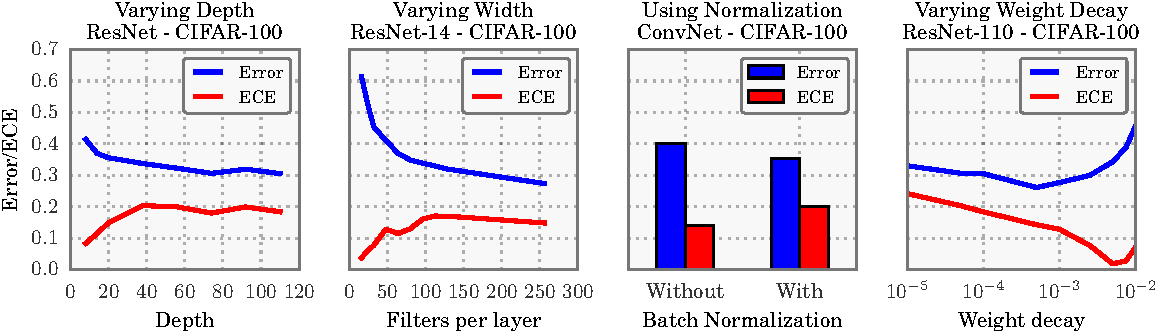
\includegraphics[width=\textwidth]{fig/factors.pdf}
  \caption{The effect of network depth (far left), width (middle left), Batch Normalization (middle right), and weight decay (far right) on miscalibration, as measured by ECE (lower is better).}
  \label{figure.factors}
  \vspace*{-2ex}
\end{figure*}

The problem we address in this paper is supervised multi-class classification with neural networks. The input $X\in\scrX$ and label $Y\in\scrY=\{1, \ldots, K\}$ are random variables that follow a ground truth joint distribution $\pi(X,Y) = \pi(Y|X) \pi(X)$.
Let $h$ be a neural network with $h(X) = (\yh, \ph)$, where $\yh$ is a class prediction and $\ph$ is its associated confidence, i.e. probability of correctness.
We would like the confidence estimate $\ph$ to be calibrated, which intuitively means that $\ph$ represents a true probability. For example, given 100 predictions, each with confidence of $0.8$, we expect that $80$ should be correctly classified.
More formally, we define \emph{perfect calibration} as
\begin{equation}
\label{perfect_calibration}
\P \left(\yh=Y\sep \ph = p\right)=p,\quad\forall p \in [0,1]
\end{equation}
where the probability is over the joint distribution.
%In the Appendix we show that if $h$ recovers the confidence of the ground truth conditional distribution, then $h$ is perfectly calibrated, which justifies this definition.
% \gp{Should we make $X$, $Y$, and $P$ lowercase?}
In all practical settings, achieving perfect calibration is impossible.
Additionally, the probability in \eqref{perfect_calibration} cannot be computed using finitely many samples since $\ph$ is a continuous random variable. This motivates the need for empirical approximations that capture the essence of \eqref{perfect_calibration}.

\paragraph{Reliability Diagrams} (e.g. \autoref{figure.complenet} bottom)
are a visual representation of model calibration \citep{degroot1983comparison,niculescu2005predicting}.
These diagrams plot expected sample accuracy as a function of confidence.
If the model is perfectly calibrated -- i.e. if \eqref{perfect_calibration} holds -- then the diagram should plot the identity function. Any deviation from a perfect diagonal represents miscalibration.

To estimate the expected accuracy from finite samples, we group predictions into $M$ interval bins (each of size $1/M$) and calculate the accuracy of each bin.
Let $B_m$ be the set of indices of samples whose prediction confidence falls into the interval $I_m = (\frac{m-1}{M},\frac{m}{M}]$.
% For samples $x_1,\ldots,x_n$, let $(\hat{y}_i,\hat{p}_i) = h(x_i)$ be the model's predictions and confidence scores for $i = 1,\ldots,n$.
% Let $M$ denote the number of bins, sometimes called the resolution \citep{stefanoonline}. We partition the interval $[0,1]$ into $M$ disjoint intervals $I_m = (\frac{m-1}{M},\frac{m}{M}]$ and define $B_m = \{ i \sep \hat{p}_i \in I_m \}$ for $m = 1,\ldots,M$. A reliability diagram (e.g., \autoref{figure.complenet}) draws bars over each interval $I_m$ whose height corresponds to the average accuracy within that bin, which we denote by
The accuracy of $B_m$ is
%
$$\acc(B_m) = \frac{1}{|B_m|}\sum_{i \in B_m}\ind(\hat{y}_i = y_i),$$
%
where $\hat{y}_i$ and $y_i$ are the predicted and true class labels for
sample $i$.
%
Basic probability tells us that $\acc(B_m)$ is an unbiased and consistent estimator of $\P(\yh = Y \mid \ph \in I_m)$. We define the average confidence within bin $B_m$ as
%
$$\conf(B_m) = \frac{1}{|B_m|}\sum_{i \in B_m}\hat{p}_i,$$
%
where $\hat{p}_i$ is the confidence for sample $i$.
%
$\acc(B_m)$ and $\conf(B_m)$ approximate the left-hand and right-hand sides of \eqref{perfect_calibration} respectively for bin $B_m$.
Therefore, a perfectly calibrated model will have $\acc(B_m) = \conf(B_m)$ for all $m \in \{ 1, \ldots, M \}$.
% As $M \! \rightarrow \! \infty$, we recover the exact definition given by \eqref{perfect_calibration}.
Note that reliability diagrams do not display the proportion of samples in a given bin, and thus cannot be used to estimate how many samples are calibrated.


\paragraph{Expected Calibration Error (ECE).}
While reliability diagrams are useful visual tools, it is more convenient to have a scalar summary statistic of calibration.
Since statistics comparing two distributions cannot be comprehensive, previous works have proposed variants, each with a unique emphasis.
One notion of miscalibration is the difference in expectation between confidence and accuracy, i.e.
%
\begin{align}
  \E_{\ph} \left[ \left| \P\left(\yh = Y \sep \ph = p\right) - p \right| \right]
  \label{eqn:miscalibration}
\end{align}
%
Expected Calibration Error \citep{naeini2015obtaining} -- or ECE -- approximates \eqref{eqn:miscalibration} by partitioning predictions into $M$ equally-spaced bins (similar to the reliability diagrams) and taking a weighted average of the bins' accuracy/confidence difference. More precisely,
\begin{equation}
\label{ece}
\text{ECE} = \sum_{m=1}^{M}\frac{|B_m|}{n}\bigg|\acc(B_m) - \conf(B_m)\bigg|,
\end{equation}
where $n$ is the number of samples.
The difference between $\acc$ and $\conf$ for a given bin represents the calibration \emph{gap} (red bars in reliability diagrams -- e.g. \autoref{figure.complenet}).
%\gp{I think we need to drive home here how to interpret ECE, since we're showing it in many graphs. We need to hammer home that it approximates our probabilistic error.}
We use ECE as the primary empirical metric to measure calibration.
See \autoref{sup:definitions} for more analysis of this metric.
%\cg{Need to rewrite this part...} For each term in the sum, $\text{acc}(B_m) \frac{|B_m|}{n}$ is its {\color{red} unbiased and consistent estimator}. On the RHS, we have $\E_{X}[\ph] = \sum_{m=1}^{M}\E_{X\in B_m}[\ph]$. And for each term in the sum, $\frac{|B_m|}{n}\hat{p}(B_m)$ is an {\color{red} unbiased and consistent estimator}. Together, we obtain an {\color{red} unbiased and consistent estimator} of
%$\E \bigg|\P\left(\yh=Y\sep \ph = p\right)-p\bigg|$.

%Alternatively,
%we know that
%$$ \P\left(Y = \yh\sep \ph\right) = \E_{X,Y} \left[\ind_{Y}(\yh)\sep \ph\right]$$
%and
%$$
%\E\left[ \E_{X,Y} \left[\ind_{Y}(\yh)\sep \ph\right]\right]
%=  \E_{X,Y} \left[\ind_{Y}(\yh)\right] = \P(\yh=Y)
%$$

\paragraph{Maximum Calibration Error (MCE).} In high-risk applications where reliable confidence measures are absolutely necessary, we may wish to minimize the worst-case deviation between confidence and accuracy:
%
\begin{equation}
  \max_{p \in [0, 1]} \left| \P\left(\yh = Y \sep \ph = p\right) - p \right|.
\end{equation}
%
The Maximum Calibration Error \citep{naeini2015obtaining} -- or MCE -- estimates this deviation. Similarly to ECE, this approximation involves binning:
\begin{equation}
\label{mce}
\text{MCE} = \max_{m \in \{1,\ldots,M\} }\left|\acc(B_m) - \conf(B_m)\right|.
\end{equation}
% Thus MCE is an empirical upper bound estimate of $|\P(\yh=Y\sep \ph = p)-p|$.
We can visualize MCE and ECE on reliability diagrams.
MCE is the largest calibration gap (red bars) across all bins, whereas ECE is a weighted average of all gaps.
For perfectly calibrated classifiers, MCE and ECE both equal 0.

\paragraph{Negative log likelihood} is a standard measure of a probabilistic model's quality \cite{friedman2001elements}. It is also referred to as the cross entropy loss in the context of deep learning \cite{bengio2015deep}. Given a probabilistic model $\hat{\pi}(Y|X)$ and $n$ samples, NLL is defined as:
%
\begin{align}
  \scrL = -\sum_{i=1}^{n}\log(\hat{\pi}(y_i|\xb_i))
\end{align}
%
It is a standard result \cite{friedman2001elements} that, in expectation, NLL is minimized if and only if $\hat{\pi}(Y|X)$ recovers the ground truth conditional distribution $\pi(Y|X)$.
